\begin{figure}
\centering
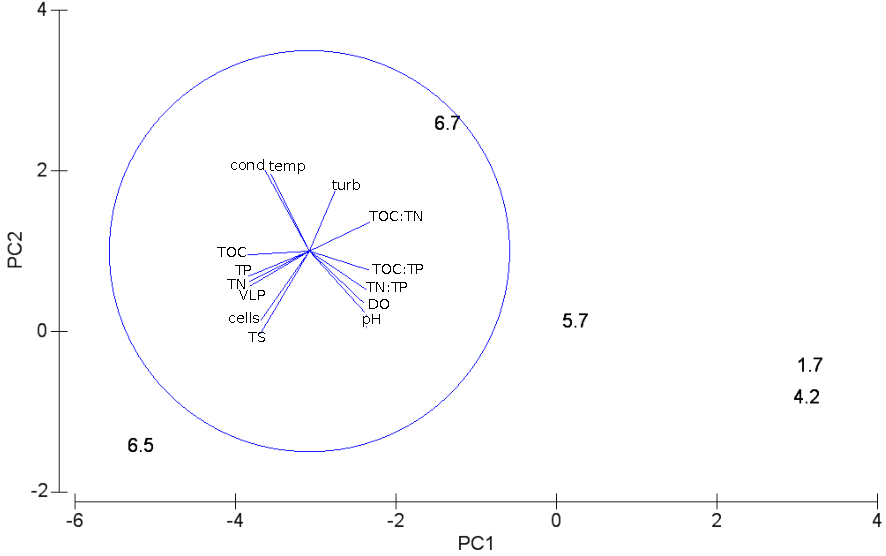
\includegraphics[width=120mm]{orglake_figures/pca.pdf}
\caption[\acs{PCA} of physico-chemical parameters]{\acs{PCA} of physico-chemical parameters and cell/\ac{VLP} counts of the Organic Lake profile. Data points are the sampling depths 1.7, 4.2, 5.7, 6.5 and 6.7 m. The overlaid vector diagram shows the relative contributions of the variables to explaining the difference between samples. PC1 explained 74.3\% and PC2 explained 14.7\% of the variation between samples. cond, conductivity; temp, temperature; turb, turbidity.}
\label{fig:pca}

\end{figure}
